% vim: set fenc=utf-8 ft=latex encoding=utf-8
% -*- mode: latex; coding: UTF-8; -*-
%!TEX root = knowledge-curation.tex
\section{Results}
\label{cha:findings}

This section presents the findings of our study that answer each research question.

\subsection{RQ-1. \rqa}
\label{cha:findings-types}


We identified five main types of knowledge from the messages from the Stack Overflow R tag and R-help mailing list:
\begin{enumerate*}[label=(\arabic*)]
\item Questions,
\item Answers,
\item Updates,
\item Flags, and
\item Comments.
\end{enumerate*}
    Each of them, with their sub-types of knowledge presented in Table~\ref{table:type-of-knowledge}. We also include the frequency of each. As we mentioned in Section~\ref{cha:methodology}, the sample of 400 questions \& answers from each channel provides a reliability of 95\% $\pm$ 5\%.
    Below we explain the five main type of knowledge, similarities and differences, when applicable and considering the potential margin of error.

    \begin{table*}[!htb]
      \centering
      \caption{Types of knowledge found in both Stack Overflow (SO) and R-help (RH), and their frequency in the analyzed sample.}
      \begin{small}
\begin{tabular}[h]{p{2.3cm}p{10.3cm}rrrrr}
 && \textbf{SO}                                                                                                                                              & \textbf{RH}  & \textbf{Prop SO} & \textbf{Prop RH}                \\
\toprule
\multicolumn{2}{@{}l}{\textbf{Questions}}\\
  \emph{How-to}                   & Ask how to do something specific.                                                                                                                        & 166          & 103              & 41.50\%        & 25.75\%        \\
  \emph{Bug/Error\-/Exception}    & Ask for a solution or reasons for a error message.                                                                                                       & 27           & 48               & 6.75\%         & 12.00\%        \\
  \emph{Discrepancy}              & Ask about an unexpected result of a specific function, process, or package.                                                                              & 53           & 88               & 13.25\%        & 22.00\%        \\
  \emph{Set-up}                   & Ask for possible ways to set up the R environment before or after deployment.                                                                            & 15           & 31               & 3.75\%         & 7.75\%         \\
  \emph{Decision help}            & Ask for advice in making a decision.                                                                                                                     & 36           & 35               & 9.00\%         & 8.75\%         \\
  \emph{Conceptual\-/Guidance}    & The user requests a conceptual clarification or guidance on topics related with R or statistics.                                                         & 48           & 49               & 12.00\%        & 12.25\%        \\
  \emph{Code reviewing}           & Ask for code review, explicitly or implicitly.                                                                                                           & 34           & 21               & 8.50\%         & 5.25\%         \\
  \emph{Non-functional}           & Ask for help (or suggestions) with a non-functional requirement such as performance, and memory usage.                                                   & 14           & 11               & 3.50\%         & 2.75\%         \\
  \emph{Future reference}         & Ask---and normally answer itself---that might not exist on the channel, but that are interesting enough to create a thread for future reference.         & 5            & 4                & 1.25\%         & 1.00\%         \\
  \emph{Other}                    & Ask for assistance unrelated to the channel or the message contains unrelated information (e.g., announcements, ideas for improvement).                  & 2            & 10               & 0.50\%         & 2.50\%         \\
                                  &                                                                                                                                                          & \textbf{400} & \textbf{400}     & \textbf{100\%} & \textbf{100\%} \\
\hline
  \multicolumn{2}{@{}l}{\textbf{Answers}}                                                                                                                                                                                                                          \\
  \emph{Redirecting}                & Provides a link to an existing solution that is not in the thread (e.g. external application, tutorial, or project).                                     & 163          & 87               & 20.20\%        & 15.03\%        \\
  \emph{Tutorial}                   & A set of steps in order to teach people how to solve the issue.                                                                                          & 105          & 15               & 13.01\%        & 2.59\%         \\
  \emph{Source code}                & Source code snippet as the solution without an extensive explanation about the answer.                                                                   & 198          & 102              & 24.54\%        & 17.62\%        \\
  \emph{Clue/Suggestion/Hint}       & Possible ways to solve the issue without solving it.                                                                                                     & 43           & 105              & 5.33\%         & 18.13\%        \\
  \emph{Alternative}                & A different approach to a solution that is related to but not exactly what is being asked for (e.g. mathematical approach, data structure modification). & 33           & 98               & 4.09\%         & 16.93\%        \\
  \emph{Explanation}                & Explains an approach that answers the question and lists steps on how to do it.                                                                          & 203          & 101              & 25.15\%        & 17.44\%        \\
  \emph{Announcement}               & Provides a notification about some artifact (e.g., packages, libraries).                                                                                 & 8            & 33               & 0.99\%         & 5.70\%         \\
  \emph{Benchmark}                  & Provides a benchmark of multiple solutions posted by others or compares different answers.                                                               & 5            & 3                & 0.62\%         & 0.52\%         \\
  \emph{Opinion}                    & Provides their own opinion or expands other answers by adding scenarios and examples.                                                                    & 49           & 35               & 6.07\%         & 6.04\%         \\
                                    &                                                                                                                                                          & \textbf{807} & \textbf{579}     & \textbf{100\%} & \textbf{100\%} \\
\hline
  \multicolumn{2}{@{}l}{\textbf{Updates}}                                                                                                                                                                                                                          \\
  \emph{Announcement}               & Announces specific events (e.g., bounties, future updates).                                                                                              & 27           & 3                & 4.40\%         & 1.21\%         \\
  \emph{Background}                 & Adds additional context to the question or answer                                                                                                        & 74           & 57               & 12.07\%        & 23.08\%        \\
  \emph{Correction}                 & Corrects format, grammar, spelling, and semantic mistakes.                                                                                               & 301          & 2                & 49.10\%        & 0.81\%         \\
  \emph{Expansion}                  & Expands the question or answer by providing scenarios or examples.                                                                                       & 116          & 83               & 18.92\%        & 33.60\%        \\
  \emph{Explanation}                & Explains or clarifies a specific point in the question or answer, such as why the user chose a specific data structure, or the meaning of a variable.    & 83           & 95               & 13.54\%        & 38.46\%        \\
  \emph{Solution}                   & The user answers their own question.                                                                                                                     & 12           & 7                & 1.96\%         & 2.83\%         \\
                                    &                                                                                                                                                          & \textbf{613} & \textbf{247}     & \textbf{100\%} & \textbf{100\%} \\
\hline
  \multicolumn{2}{@{}l}{\textbf{Flags}}                                                                                                                                                                                                                            \\
  \emph{Off-topic/opinion}          & Identify questions that are unrelated to the channels' interests or which answers are seek opinion.                                                      & 22           & 19               & 27.16\%        & 35.19\%        \\
  \emph{Not an answer}              & Emphasize \textit{alternative answers} out of the scope of the question, or to identify that a solution does not answer the question.                    & 0            & 27               & 0.00\%         & 50.00\%        \\
  \emph{Repeated question}          & Notifies user that question has been answered previously.                                                                                                & 48           & 8                & 59.26\%        & 14.81\%        \\
  \emph{Too localized}              & Questions that are too specific and might not help any future reader.                                                                                    & 6            & 0                & 7.41\%         & 0.00\%         \\
  \emph{Unclear}                    & Questions that are difficult to understand.                                                                                                              & 5            & 0                & 6.17\%         & 0.00\%         \\
                                    &                                                                                                                                                          & \textbf{81}  & \textbf{54}      & \textbf{100\%} & \textbf{100\%} \\
\hline
  \multicolumn{2}{@{}l}{\textbf{Comments}}                                                                                                                                                                                                                     \\
  \emph{Clarification}          & Provides (or requests) additional information about a question or answer.                                                                                & 98           & 28               & 17.44\%        & 10.49\%        \\
  \emph{Expansion}              & Provides additional information.                                                                                                                         & 127          & 65               & 22.60\%        & 24.34\%        \\
  \emph{Correction/alternative} & Suggests a change to a question or answer, offers an alternative solution or a correction.                                                               & 102          & 89               & 18.15\%        & 33.33\%        \\
  \emph{Compliment/criticism}   & Posts something good, offers thanks, provides an opinion or criticise someone.                                                                           & 157          & 52               & 27.94\%        & 19.48\%        \\
  \emph{External reference}     & References an external resource.                                                                                                                         & 78           & 33               & 13.88\%        & 12.36\%        \\
                                &                                                                                                                                                          &\textbf{562}  & \textbf{267}     & \textbf{100\%} & \textbf{100\%} \\
  \bottomrule
        \end{tabular}
      \end{small}
      \label{table:type-of-knowledge}
\vspace{-3mm}
    \end{table*}

\paragraph*{Questions and Answers}
    Questions express one or more problems or doubts faced by an user in Stack Overflow or R-help, whereas answers represent solutions to questions.  We observed that the types of questions in \SO are more specific than those in \RH, and are more likely to be tutorials. Also, \SO has more answers per question---2 per question compared to 1.4 of \RH. However, \RH questions tend to offer more suggestions or alternatives than \SO answers. This might be a result of the narrowness of \SO questions.

\paragraph*{Updates}
	A modification to a question or answer.
	On the R-help mailing list, updates are not easily identifiable as the communication is presented as plain text emails.
	Therefore, for \RH we defined updates  as \emph{follow-ups by an author who had already posted once to a thread}.

	In Stack Overflow updates are presented in two ways:
	\begin{description}[itemsep=3pt, topsep=2pt, leftmargin=3em, parsep=0pt]
		\item[Labelled updates] are explicitly shown in the body of questions or answers next to a label that identifies the update (e.g., edit, update, and p.s.).
		When multiple update labels appear in a message, each label is accompanied by a number (e.g., \textit{``[Edit 1:]''} {\footnotesize URL:  \url{http://goo.gl/ptYAG0}{Q1452235}}), by a date (e.g., \textit{``Edit/Update (April 2011):''} {\footnotesize URL:  \url{http://goo.gl/ptYAG0}{Q1452235}}), or by a bulleted list (e.g., ``EDIT: - anova... -drop1...'' {\footnotesize URL:  \url{http://goo.gl/sQiq0M}{Q7273695}})

		\item[Non-labelled updates] are only visually recognizable through the message history system. The only indication of the change is a box at the end of the message that contains the user who performed the change and the date when it happened.
	\end{description}

	Depending of the type of update, the usage is different.
	Non-labelled updates are mainly used to correct format, grammar, spelling, and semantic mistakes, or to incorporate explanations, examples, and suggestions without changing the meaning of the question or answer. Labelled updates are for everything else. Regarding their frequency,  the \SO sample had 2.5 more Updates than \RH.
Corrections are more common in \SO (almost 50\%), while in \RH updates are usually adding extra information to the thread in various forms (Background, Expansion and Explanation).

\paragraph*{Flags}

	On Stack Overflow, a flag is a mechanism to get a moderator's attention.
	Flags can accomplish different objectives: to mark messages as spam, rude or abusive behaviour; and, to identify duplicate questions, off-topic messages, unclear questions, opinion-based questions, and low-quality answers.
	Depending of the type of the flag, threads can be closed or users can lose reputation point.
    On the R-help mailing list, the concept of flag does not exist. 
    Based on the definition of flags on Stack Overflow, we defined flags as \emph{messages used to call the attention of other community members}.
    Thus, we found that flags on the R-help mailing list are used to keep a healthy community, promote discussion, and call the attention of community members to certain issues.
    Given our definition, flags might be used by the person who asked or answered a question (in \SO authors of a question cannot add flags to it).
    Due to the unstructured form of messages on the R-help mailing list, flags can be mixed among the text of answers, comments, questions and updates.
	Flags in the R-help mailing list do not constrain users to answer questions, or to clarify what it is already asked.

In terms of their frequency, \SO uses flags primarily to mark repeated questions; in contrast, \RH uses them to indicate that a previous answer is incorrect. \SO had 1.5 times more Flags than \RH.


\paragraph*{Comments}
In Stack Overflow, comments are \textit{``temporary `Post-It' notes left on a question or answer..''}\footnote{\url{http://stackoverflow.com/help/privileges/comment}}.
	Comments are located below each question or answer, and can be used as a follow-up to questions, to answer a question, or to clarify a question.
	On the R-help mailing list, we defined comments as messages written to \emph{improve an answer in response to an incomplete question, or as a follow-up on a discussion}.
	Most importantly, messages should be written by a \emph{different person than the author of the question or answer} to which they are responding.
	In this context, the difference between an update and a comment is the motivation of the user who wrote the message and the author of the message.
	The format of the message in Stack Overflow and the R-help mailing list, permits participants to ask multiple questions in the same thread.
	Therefore, the categorizations of knowledge presented in this section are non-mutually exclusive.
        Regarding their frequency, the statistical differences were that in \SO comments are less likely to be Corrections/Alternative; also, \SO had 2.1 times more Comments than \RH.

\subsection{RQ-2. How is knowledge constructed on Stack Overflow and the R-help mailing list?}
\label{sec:rq2}

    Through our analysis, we identified two different approaches for constructing knowledge:

        \noindent\textbf{Participatory knowledge construction} are answers created through the cooperation of multiple users in the same thread.
        Participants complement each other's questions by providing pros and cons about the answer, different viewpoints, or additional context and examples.
        This is comparable with the concept of team in which people work together in a cooperative way for the same objective.

\noindent        \textbf{Crowd knowledge construction} leverages the experiences of many users; each user contributes its own explanations and practices adding variety to the pool of solutions.
        This is comparable with the concept of group in which people work towards the same objective but not necessarily together.
        Participants can vote over others ideas, but the idea is not constructed through a discussion process.
    
    On the R-help mailing list, participatory knowledge takes place when:
    \begin{enumerate*}[label=(\arabic*)]
    \item previous answers are included in the actual answer and it is possible to infer a link between them; or
    \item when a in the message contains a direct reference to other answers or authors.
    \end{enumerate*}
    Figure \ref{fig:ML-PK1} depicts two examples of the way participatory knowledge occurs on the R-help mailing list:
    direct citation of the author of a previous answer (top), and inferable links between answers (right).

    
    \begin{figure}[!htb]
        \centering
        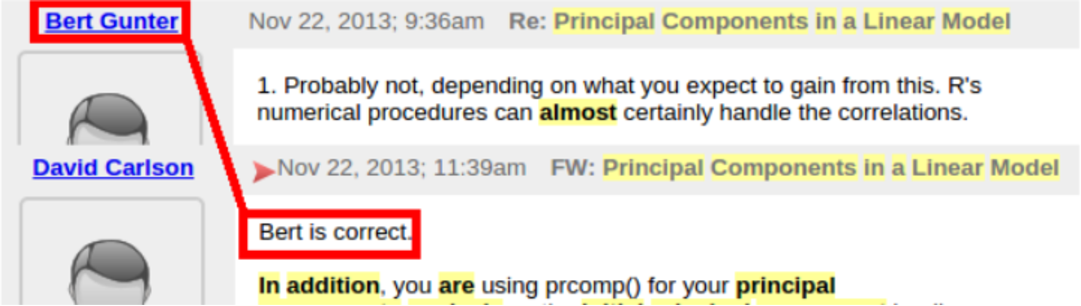
\includegraphics[width=\columnwidth]{Figures/ML-PKimg2}
        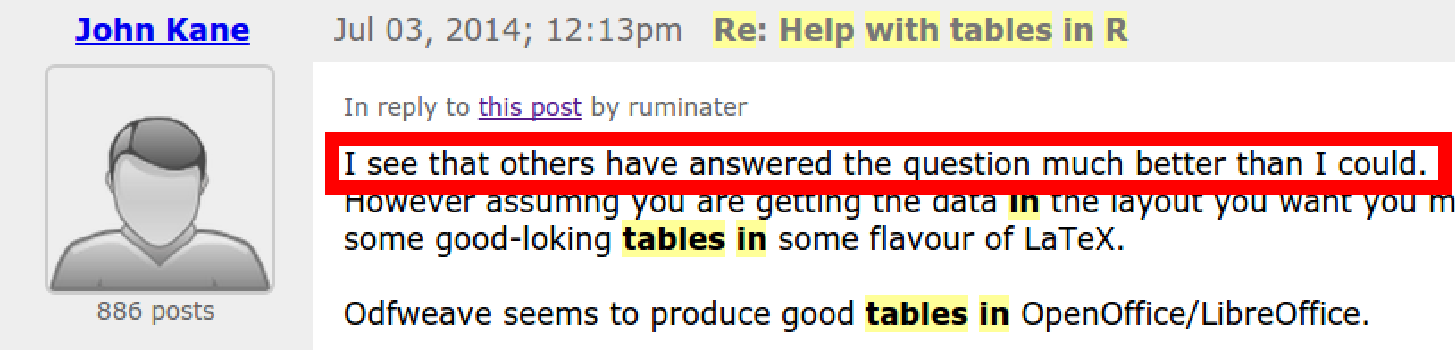
\includegraphics[width=\columnwidth]{Figures/ML-PKimg11}
        \caption[Participatory knowledge on the R-help mailing list.]{Participatory knowledge on the R-help mailing list.}
        \label{fig:ML-PK1}
\vspace{-3mm}
    \end{figure}

    On Stack Overflow, participatory knowledge takes place when:
    \begin{enumerate*}[label=(\arabic*)]
    \item it is possible to infer a link between answers, via either a direct or indirect reference; or
    \item comments complement the answer, or directly cite another author.
    \end{enumerate*}

    On Stack Overflow, participatory knowledge happens in different places, perhaps as a consequence of its rich interface.
    We observe this phenomena, when a user answers a question and directly cites or links to the author of another answer in the thread, or when a user cites the author of a question or answer in a comment made on that question or answer, by including more information, or by suggesting that the answer provided is an additional solution.
    Figure \ref{fig:SO-PK1} depicts an example of participatory knowledge in Stack Overflow: the author participate in the comments to help another user when the answer is not sufficient for a particular case.
    In the comment, the user references another authors and answer.

    \begin{figure}[!htb]
        \centering
        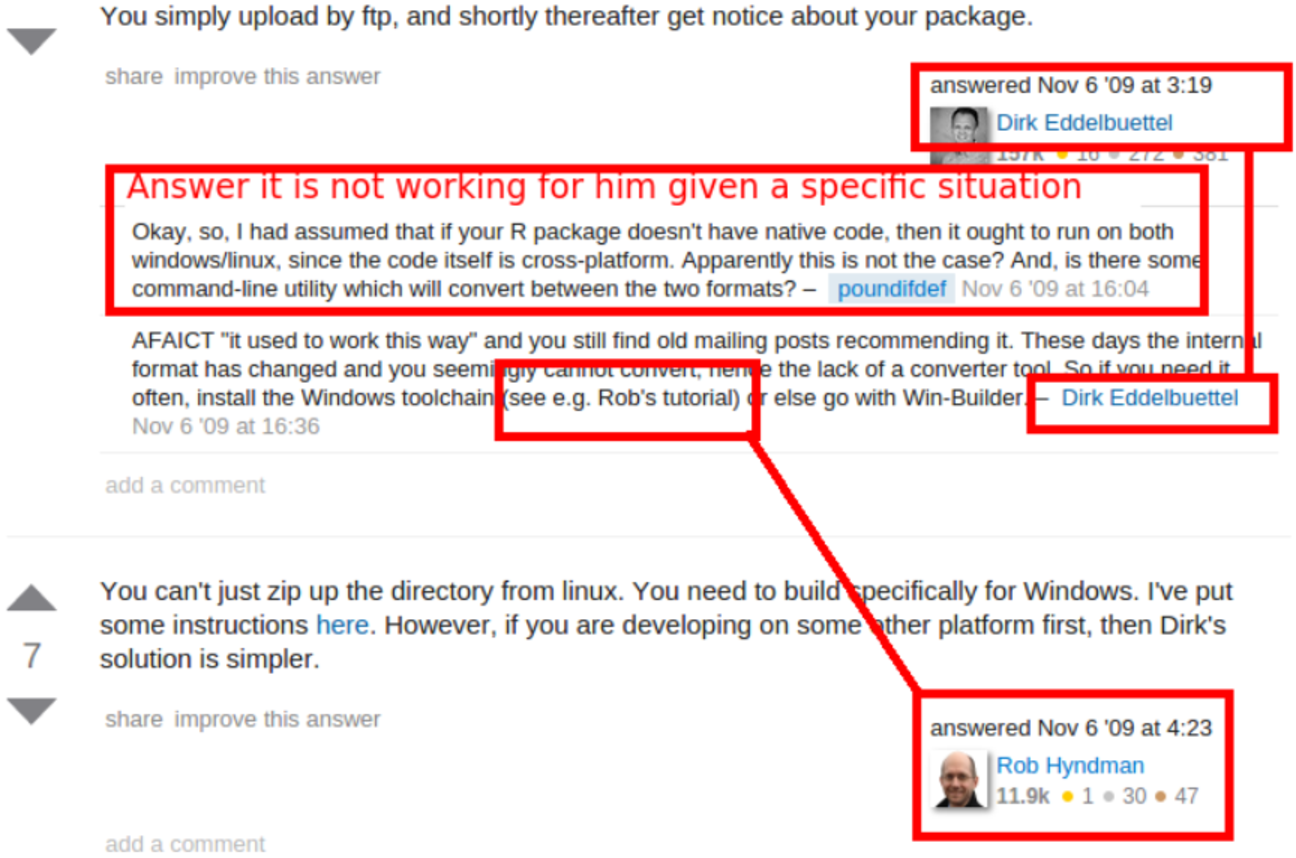
\includegraphics[width=\columnwidth]{Figures/SO-PKimg5}
        \caption{Example of participatory knowledge on Stack Overflow.}
        \label{fig:SO-PK1}
\vspace{-3mm}
    \end{figure}

    Crowd knowledge construction is observable when:
    \begin{enumerate*}[label=(\arabic*)]
    \item there is not a direct or inferable reference between answers,
    \item answers are a variation of one of the answers on the thread.
    \end{enumerate*}
    Figure \ref{fig:CKC_MLSO} depicts an example of how crowd knowledge construction is visible on Stack Overflow.
    As can be seen from the figure, there are two of the three answers that provided a repeated solution.

    \begin{figure} [!htb]
        \centering
        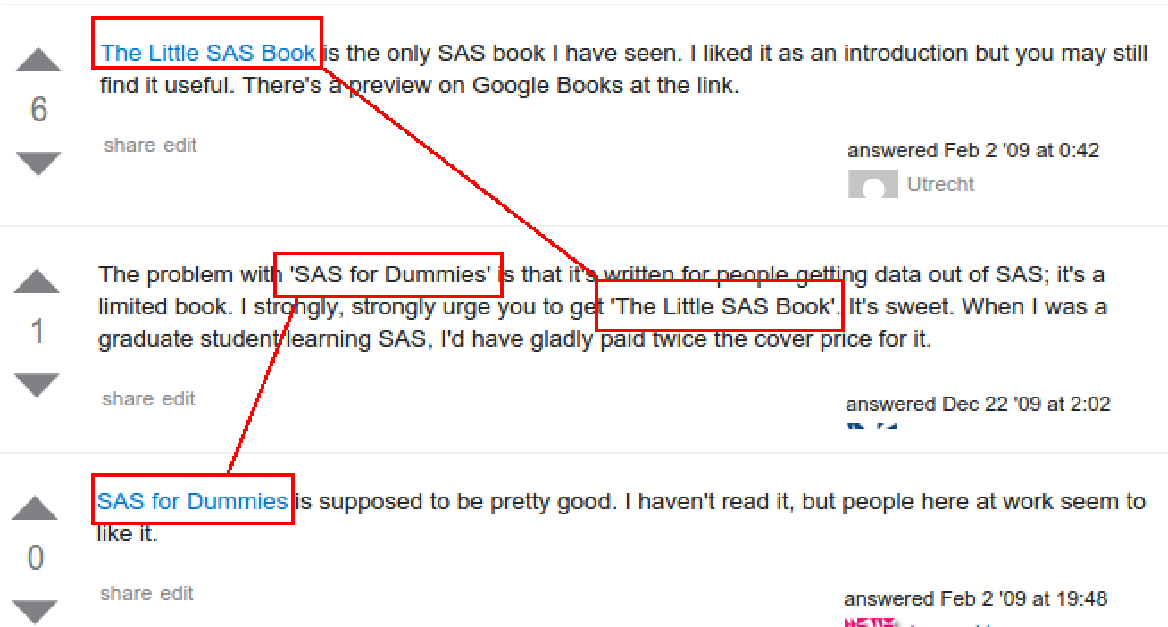
\includegraphics[width=\columnwidth]{Figures/SO-CSimg2}
        \caption{Example of how crowd knowledge construction occurs.}
        \label{fig:CKC_MLSO}
\vspace{-3mm}
    \end{figure}

\subsection{RQ-3. Why do certain users post to both Stack Overflow and the R-help mailing list}

Based on the responses from the survey, we identified that being active on both channels brings benefits to those asking and answering questions:

\begin{packed_enum}
\item \textbf{Find a better answer:} One channel might provide a better answer than the other.
\item \textbf{Support follow-up questions:} We found that it is not uncommon to use the mailing list to have follow-up discussions on specific \SO
  questions. These discussions were mode specific about the rational for an answer.\dmg{here I am speculating this is what carlos meant}
\item \textbf{Speeds up answers:} Users ask the same question on both channels to speed up getting an answer, and to get more points of view. However, this behaviour s not encouraged by the community as it is deemed impolite.\dmg{reference}
\end{packed_enum}

 Also, users commented on the reasons why they prefer one channel over the other:

\noindent\textbf{\SO}:
    The reported benefits of using Stack Overflow were: gaining peer recognition, it has a friendly and rich interface, answers are straight to the point, it is
    easy to search and questions are usually answered faster.
    However, the drawbacks of using Stack Overflow include: the abundance
    of related questions; certain level of experience is required to understand some of the answers, and \SO strict rules that only allow questions and their answers. In
    general, \SO does not allow discussions to take place, including questions that ask for opinions.

\noindent\textbf{\RH}:
The benefits of using \RH include: the convenience of just handling email; following the mailing list provides awareness of and leads towards
learning new topics; the participation of highly experienced
users; and its flexibility regarding the topics that one can discuss.  The disadvantages that were reported include: sometimes there can be aggressive
behaviour; searching the archives is not easy; and emails lack categorization, which makes it difficult organize given the massive volume of information.

%%% Local Variables:
%%% mode: latex
%%% TeX-master: "knowledge-curation.tex"
%%% End:
